\newpage
\subsection{UC4 - Modifica Grafico}
\label{subsec:uc4}

%TODO: Add correct image
\begin{figure}[h]
    \centering
    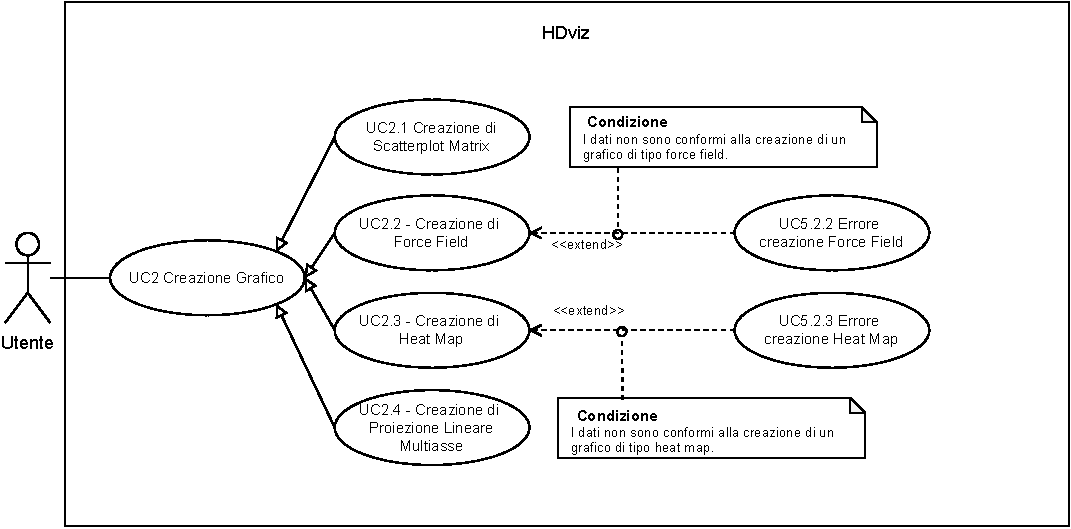
\includegraphics[width=0.8\textwidth]{componenti/casi-duso/diagrammi/UC2.pdf}
    \caption{Diagramma rappresentante UC2}
    \label{fig:UC4}
\end{figure}


\begin{itemize}
    \item \textbf{Descrizione}: L’utente modifica la visualizzazione del grafico precedentemente costruito
                                e ne vede le modifiche.
	
    \item \textbf{Attore primario}: Utente.
    
    \item \textbf{Precondizione}:   Nel programma è stato importato un dataset dotato di metatag per ogni
                                    colonna dei dati ed è stato costruito un grafico di una tipologia scelta dall'utente.

    \item \textbf{Postcondizione}:  Viene aggiornato il grafico costruito e visualizzato con i nuovi parametri.

	\item \textbf{Scenario principale}:
		\begin{enumerate}
			\item L'utente decide di modificare il grafico corrente.
			\item L'utente effettua le modifiche desiderate.
            \item L'utente conferma le modifiche apportate selezionando il pulsante di conferma.
        \end{enumerate}

    \item \textbf{Scenario alternativo}:
        \begin{enumerate}
            \item L'utente decide di annullare le modifiche effettuate (UC4.5) al posto di confermarle.   
            \item Le modifiche vengono scartate e viene ripristinata la visualizzazione del grafico prima delle modifiche.
        \end{enumerate}
    
\end{itemize}


\subsection{UC4.1 Modifica Scatterplot Matrix}





\subsection{UC4.2 Modifica Force Field}
% TODO: Create image for force field graph.
\begin{figure}[h]
    \centering
    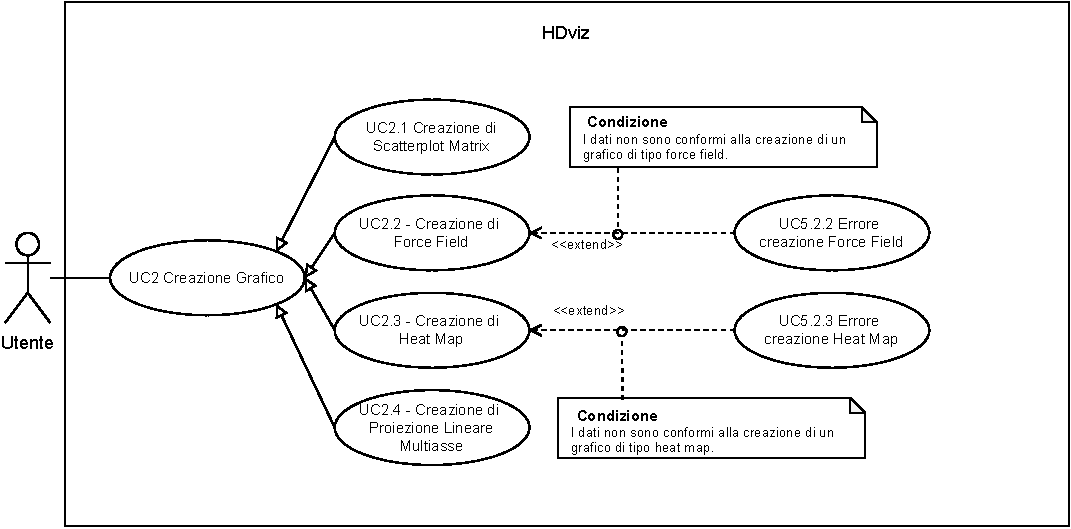
\includegraphics[width=0.8\textwidth]{componenti/casi-duso/diagrammi/UC2.pdf}
    \caption{Diagramma rappresentante UC2}
    \label{fig:UC2}
\end{figure}


\begin{itemize}
    \item \textbf{Descrizione}: L’utente vuole modificare la visualizzazione del grafo Force Field
                                costruito dal dataset corrente.
	
    \item \textbf{Attore primario}: Utente.
    
    \item \textbf{Precondizione}:   Il grafico precedentemente costruito dal dataset corrente è un Force Field.

    \item \textbf{Postcondizione}:  Viene aggiornato il grafico costruito e visualizzato con i nuovi parametri.

	\item \textbf{Scenario principale}:
		\begin{enumerate}
            \item L'utente apporta le modifiche desiderate tra quelle offerte dal Force Field.
        \end{enumerate}
\end{itemize}

\subsubsection{UC4.2.1 Modifica posizione dei nodi}

\begin{itemize}
    \item \textbf{Descrizione}: L’utente vuole esplorare meglio i dati e decide di 
                                modificare la posizione dei nodi del grafo, trascinandoli con il 
                                cursore nell'area definita dal grafico.
	
    \item \textbf{Attore primario}: Utente.
    
    \item \textbf{Precondizione}:   Il grafico precedentemente costruito dal dataset corrente è un Force Field.
    \item \textbf{Postcondizione}:  Viene modificata la posizione dei nodi del grafo nel grafico.

	\item \textbf{Scenario principale}:
        \begin{enumerate}
            \item L'utente tiene premuto il tasto di selezione e trascina il cursore sponstando il nodo nello spazio del grafico.
            \item Il grafico muove i suoi punti mantentendo le connessioni tra i nodi.
        \end{enumerate}
\end{itemize}

\subsubsection{UC4.2.2 Modifica dell'algoritmo delle distanze}

\begin{itemize}
    \item \textbf{Descrizione}: L’utente decide di cambiare l’algoritmo usato per il calcolo delle distanze.

	
    \item \textbf{Attore primario}: Utente.
    
    \item \textbf{Precondizione}:   Il grafico precedentemente costruito dal dataset corrente è un Force Field.
    \item \textbf{Postcondizione}:  Viene modificata la distanza tra i nodi del grafo nel grafico.

	\item \textbf{Scenario principale}:
        \begin{enumerate}
            \item L'utente seleziona il menu delle distanze e seleziona uno degli algoritmi presentati nel menù.
            \item Il grafico modifica la distanza tra i nodi secondo l'algoritmo scelto.
        \end{enumerate}
\end{itemize}

\subsubsection{UC4.2.3 Modifica intensità forza attrattiva tra nodi}

\begin{itemize}
    \item \textbf{Descrizione}: Per poter visualizzare meglio i cluster di dati l’utente 
                                decide di scalare la forza di attrattiva tra i nodi.

	
    \item \textbf{Attore primario}: Utente.
    
    \item \textbf{Precondizione}:   Il grafico precedentemente costruito dal dataset corrente è un Force Field.
    \item \textbf{Postcondizione}:  Viene modificata l'intensità della forza attrattiva tra i nodi del grafico.

	\item \textbf{Scenario principale}:
        \begin{enumerate}
            \item L'utente seleziona la barra intensità e trascinando il cursore sulla barra varia l’intensità.
            \item Il grafico modifica l'intensità della forza secondo il valore selezionato.
        \end{enumerate}
\end{itemize}

\subsubsection{UC4.2.4 Modifica proprietà di un nodo per dimensione}

\begin{itemize}
    \item \textbf{Descrizione}: Per poter visualizzare meglio i cluster di dati l’utente 
                                decide di scalare la forza di attrattiva tra i nodi.

	
    \item \textbf{Attore primario}: Utente.
    
    \item \textbf{Precondizione}:   Il grafico precedentemente costruito dal dataset corrente è un Force Field.

    \item \textbf{Postcondizione}:  Viene modificato lo stile dei nodi per una determinata dimensione del grafico costruito.

	\item \textbf{Scenario principale}:
        \begin{enumerate}
        
            \item L'utente seleziona il menu delle dimensioni.
            \item L'utente seleziona la dimensione di interesse.
            \item L'utente manipola le proprietà che gli interessano.
            \item Il grafico mostra i nuovi nodi per la dimensione selezionata.
                
        \end{enumerate}
\end{itemize}


\subsubsection{UC4.2.4.1 Modifica colore}

\begin{itemize}
    \item \textbf{Descrizione}: L'utente decide di modificare il colore di nodi relativi ad una dimensione.

	
    \item \textbf{Attore primario}: Utente.
    
    \item \textbf{Precondizione}:   L'utente ha selezionato l'opzione di modifica delle proprietà dei nodi per dimensione (UC4.2.4).
    \item \textbf{Postcondizione}:  Viene aggiornato il colore dei nodi della dimensione selezionata.

	\item \textbf{Scenario principale}:
        \begin{enumerate}
            \item L'utente seleziona il nuovo colore da assegnare ai nodi tra quelli resi disponbili.
        \end{enumerate}
\end{itemize}

\subsubsection{UC4.2.4.2 Modifica raggio}

\begin{itemize}
    \item \textbf{Descrizione}: L'utente decide di modificare il raggio di nodi relativi ad una dimensione.
	
    \item \textbf{Attore primario}: Utente.
    
    \item \textbf{Precondizione}:   L'utente ha selezionato l'opzione di modifica delle proprietà dei nodi per dimensione (UC4.2.4).
    \item \textbf{Postcondizione}:  Viene aggiornato il raggio dei nodi della dimensione selezionata.

	\item \textbf{Scenario principale}:
        \begin{enumerate}
            \item L'utente fa variare il raggio dei nodi mediante uno slider.
        \end{enumerate}
\end{itemize}

\subsubsection{UC4.2.4.3 Modifica opacità}

\begin{itemize}
    \item \textbf{Descrizione}:  L'utente decide di modificare l'opacità dei nodi relativi ad una dimensione.

	
    \item \textbf{Attore primario}: Utente.

    \item \textbf{Precondizione}: L'utente ha selezionato l'opzione di modifica delle proprietà dei nodi per dimensione (UC4.2.4).
    \item \textbf{Postcondizione}:  Viene aggiornata l'opacità dei nodi della dimensione selezionata.

	\item \textbf{Scenario principale}:
        \begin{enumerate}
            \item L'utente fa variare l'opacità dei nodi mediante uno slider.
        \end{enumerate}
\end{itemize}


\subsection{UC4.5 Annulamento delle modifiche}

\begin{itemize}
    \item \textbf{Descrizione}: L'utente decide di scartare le modifiche fatte nella corrente selezione di modifica.

    \item \textbf{Attore primario}: Utente.
    
    \item \textbf{Precondizione}:   L'utente ha selezionato la voce di Modifica Grafico dal menu.
    \item \textbf{Postcondizione}:  Viene ripristinato il grafico ai parametri precedenti della selezione e visualizzato.

	\item \textbf{Scenario principale}:
        \begin{enumerate}

            \item L'utente seleziona il pulsante "Annulla modifiche".
            \item HDviz ripristina i parametri del grafico ai valori precedenti alla selezione del menu di modifica.
        
        \end{enumerate}
\end{itemize}



